\documentclass[]{standalone}
\usepackage{mathptmx}
%\renewcommand{\familydefault}{\rmdefault}
\usepackage[T1]{fontenc}
\usepackage[latin9]{inputenc}
\usepackage{siunitx}
\usepackage{array}
\usepackage{amsmath}
\usepackage{ifthen}
\usepackage{pgfplots}
\pgfplotsset{compat=1.14}
\usepackage{titling, graphicx}
\usepackage{tikz}
\usepackage{upgreek}
\usepackage{amsmath,amsthm}
\usepackage{strtikz}
\usetikzlibrary{shapes,arrows.meta,intersections,graphs,graphs.standard,math,fit}
\usetikzlibrary{calc,intersections,through,backgrounds}
\usetikzlibrary{decorations.pathmorphing, decorations.markings,decorations.pathreplacing}


\begin{document}
\def \fsize {\footnotesize}
\begin{tikzpicture}
\rotspringlocal[startx = 0cm,
  starty = 0cm,
  start rigid length = 2cm,
  end rigid length = 2cm,
  dof arrow ratio = 0.2,
  dof fontsize = \tiny,
  rotation = 30,
  start angle = 100,
  end angle = 260,
  radius ratio = 0.80,
  cycle number = 5,
  cycle diameter = 0.0005cm,
  rigid line thickness = 2pt,
  spring line thickness = 1pt,
  spring stiffness = $k_\theta$,
  spring mode = 1,
  spring coefficient = 0.75,
  stiffness location = above left,
  stiff location offset = 2pt,
  rigid left text = \scriptsize{$L_1=0$},
  rigid right text = \scriptsize{$L_2=0$},
  rigid text offset = -2pt]
%\draw (0,0) -- (1cm,1cm);
\end{tikzpicture}
\end{document}